\section{Kalman-Filter}

\subsection{Beweggründe zur Nutzung des Kalmanfilters}
Der Kalmanfilter zum Fahrspurverfolgung wurde implementiert, um einige Schwächen des 1. Ansatzes zur Erkennung der Straßenmarkierungen zu beheben.
\begin{itemize}
\item Durch den prinzipbedingt als konstant angenommenen Abstand der rechten, mittleren und linken Linie sollte ein \glqq Ineinanderlaufen \grqq der \gls{acr:roi} zur Erkennung selbiger verhindert werden.
\item Da nur kleine Teile des Bildes mit eine Kantendetektor bearbeitet werden und keine Binarisierung der Filterantwort stattfinden muss, sollte der Algorithmus schneller ablaufen können.
\end{itemize}

\subsection{Vorteile}
Durch den Einsatz der \gls{glos:scanline}s anstatt einer Verwendung des \gls{acr:ransac}-Algorithmus im Zusammenhang mit Maskierung der entsprechenden Bildausschnitte läuft die Bildverarbeitung ca. um Faktor 5 schneller ab.

\subsection{Probleme}
Die Vorhersage des Folgezustands durch das Zustandsraummodell \eqref{eq:nextstatemappingmatrix} sind oft so schlecht, dass \gls{glos:scanline}s Punkte einer falschen Fahrbahnmarkierung erkennen. Somit \glqq wandert \grqq das im Zustandsvektor \gls{lat:statevector} repräsentierte Polynom durch die fehlerhafte Korrektur von der Mittellinie, welche es repräsentieren soll, zu einer der Randlinen und schließlich völlig abseits der Fahrbahn (siehe Abbildung \ref{fig:evaluation:kalman:weggezogen}).

\begin{figure}[ht] % [htb]
	\centering
	\subfloat[][]{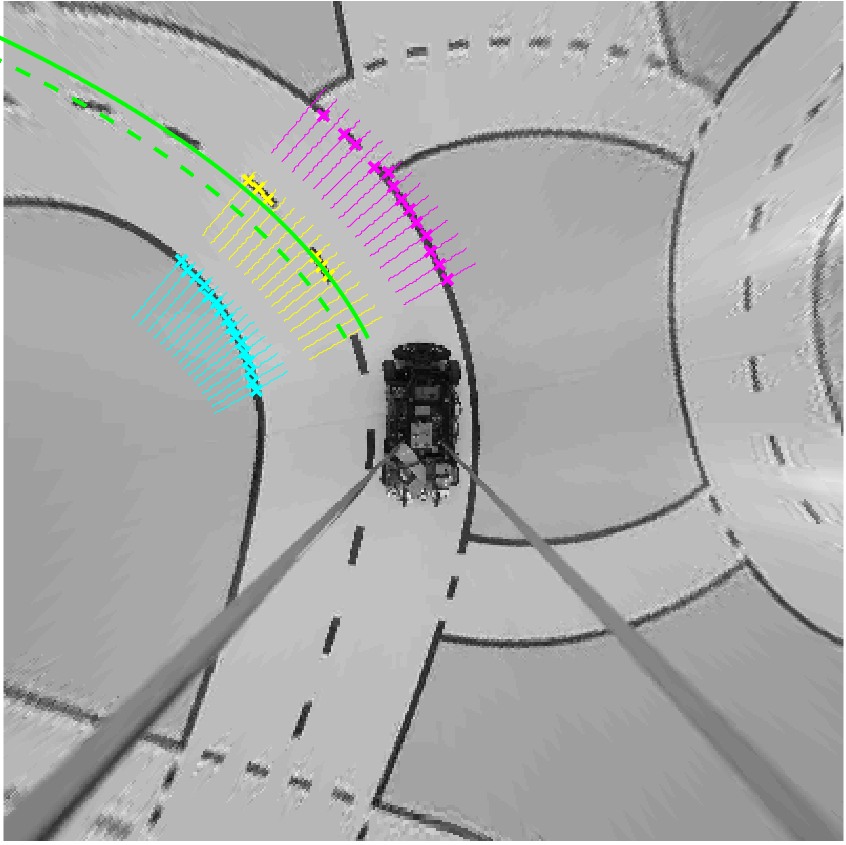
\includegraphics[width=0.45\textwidth]{evaluation_kalman_weggezogen_1}}
	\qquad
	\subfloat[][]{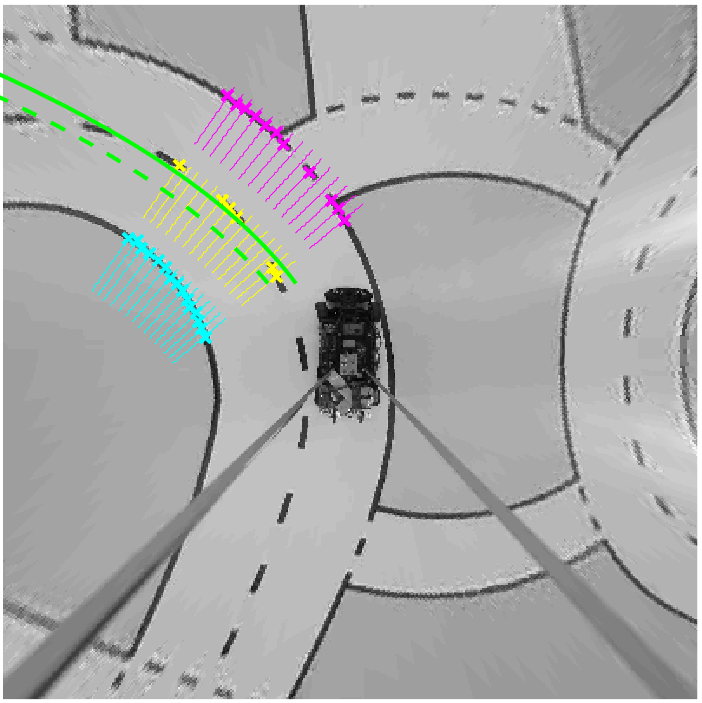
\includegraphics[width=0.45\textwidth]{evaluation_kalman_weggezogen_2}}
	\subfloat[][]{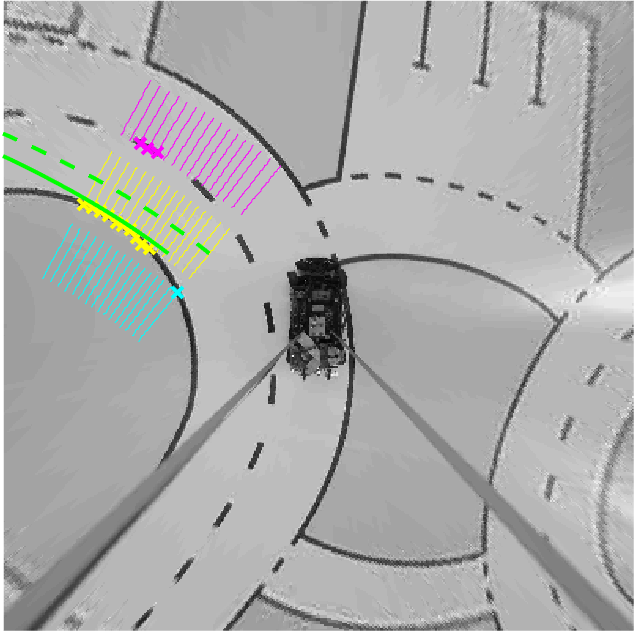
\includegraphics[width=0.45\textwidth]{evaluation_kalman_weggezogen_3}}
	\qquad
	\subfloat[][]{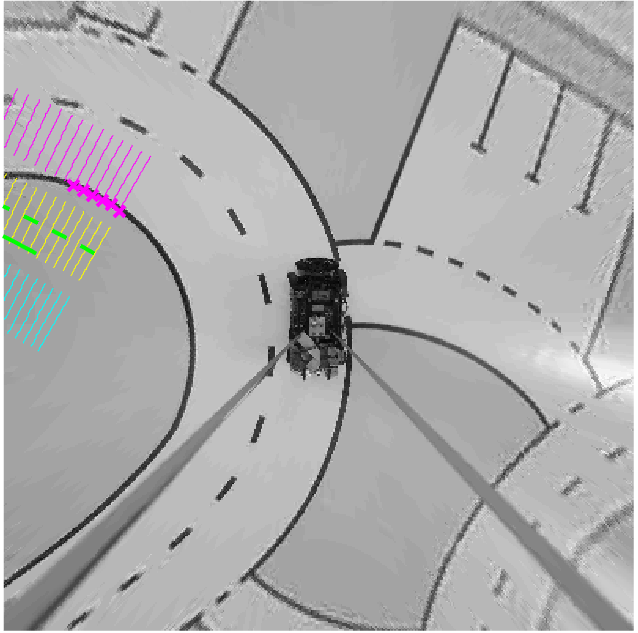
\includegraphics[width=0.45\textwidth]{evaluation_kalman_weggezogen_4}}
	\subfloat[][]{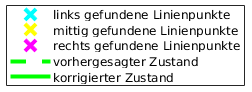
\includegraphics[width=0.45\textwidth]{evaluation_kalman_weggezogen_legende}}
	\caption{\glqq Weglaufen \grqq des Kalmanfilter-Zustands durch ungenügende Vorhersage}
	\label{fig:evaluation:kalman:weggezogen}
\end{figure}

Eine Variante dieses Phänomen zu verhindern, wäre eine Verbesserung des Zustandsraummodells. 
Ein Einbinden des Lenkwinkels, der Winkelgeschwindigkeit oder Orientierung des Fahrzeugs als Eingang \gls{lat:inputvector} wäre theoretisch möglich. Da der Zusammenhang zwischen diesen Größen und den Elementen des Zustandsvektors \gls{lat:statevector} leider nicht trivial ist und keine Literaturquelle vorliegt in der ein Zustandsraummodell mit diesen Eingangsgrößen gezeigt ist, wurde jedoch vorerst darauf verzichtet. In der Literatur wird beim Nutzung eines Kalmanfilters zur Fahrspurverfolgung oft sogar gänzlich von einer Vorhersage abgesehen, d.h. \(\gls{lat:systemmatrix}=\gls{lat:unitmatrix}\) \autocite{limRiverFlowLane2012}.

Eine weitere Möglichkeit zur Verbesserung der Performance des vorgeschlagenen Algorithmus stellt die Erhöhung der Bildrate dar. Hierdurch kann eine ungenaue Vorhersage durch häufige Korrektur ausgeglichen werden. Durch eine noch effizientere Implementierung, Parameteroptimierung sowie eine Verkleinerung der Auflösung und/oder des Bildausschnittes könnte dies erzielt werden. Da der in \ref{sec:fahrspurerkennung:riverflow} beschriebene Ansatz ohne jegliche Optimierung im jetzigen Testszenario weitaus bessere Ergebnisse lieferte, wurde jedoch keine weitere Verfeinerung dieser Methode vorgenommen.

Einen weiteren signifikanten Nachteil stellt wie in REFERENZ die Modellierung der Fahrspur durch ein Polynom 3. Grades \(\gls{y}(\gls{x})\) dar, welches schon eine \(90\deg\)-Kurve sehr schlecht approximieren kann, da dessen Anstieg unendlich werden müsste. Die volle Sichtweite des Fahrzeugs kann somit nicht genutzt werden (siehe z.B. \ref{fig:evaluation:kalman:weggezogen}).
